\def\ttt{\texttt}
\def\trm{\textrm}
\def\tbf{\textbf}
\def\tsf{\textsf}

\newcommand{\itc}[1]{\textit{\it #1\/}}
\newcommand{\tup}[1]{\langle #1 \rangle}
\newcommand{\qt}[1]{\textrm{``}#1\textrm{''}}

\def\ttob{\texttt{\symbol{`\{}}}
\def\ttcb{\texttt{\symbol{`\}}}}
\newcommand{\ttc}[1]{\ttob{#1}\ttcb}

\newcommand{\src}{\ensuremath{\mathit{src}}}
\newcommand{\sink}{\ensuremath{\mathit{sink}}}
\newcommand{\TODO}[1]{\textcolor{red}{\tbf{TODO:} #1}}
\newcommand{\notes}[1]{\textcolor{red}{#1}}
\newcommand{\lujo}[1]{\notes{$\stackrel{\hbox{\tiny Lujo}}{\hbox{\tiny
        says}}$: #1}}
\newcommand{\limin}[1]{\notes{$\stackrel{\hbox{\tiny Limin}}{\hbox{\tiny says}}$: #1}}
\newcommand{\wek}[1]{\notes{$\stackrel{\hbox{\tiny Will}}{\hbox{\tiny says}}$: #1}}

\def\lxor{\oplus}
\def\impl{\Rightarrow}
\def\bicond{\Leftrightarrow}

\def\True{\ttt{true}}
\def\False{\ttt{false}}
\def\ds{\displaystyle}

\nonfrenchspacing



%%%%%%%%%%%%%%%%%%%%%%%%%%%%%%%%%%%%%%%%%%%%%%%%%%%%%%%%%%%%%%%%%%

\spacing{1.07}

\chapter{Introduction} 
\label{sec:introduction}
Mobile devices such as smartphones and tablets are 
ubiquitous. The application environments on these devices implement
a marketplace model, in which application developers publish
apps which users can conveniently download and install
from app stores. These apps can
potentially access a variety of sensitive information, such as
a user's location, contacts, and the unique identifier of the
phone (IMEI). Applications such as social networking and banking
apps can additionally collect and store a large amount of sensitive
data. A significant concern in this setting is exfiltration of
sensitive data, which may violate
users' privacy and allow undesired tracking of users' behavior. 
Indeed, it has been shown that popular Android apps leak sensitive information, including location, IMEI number, phone number, and the SIM card ICC-ID~\cite{enck2010taintdroid}. 
%\notes{cite some example bad behavior from the news or traintdroid?}
%Another example is that a Skype app was discovered to leak profile and IM information \cite{wired2011skypes} which other apps could read. 
%In 2014, a malicious app which allows remote access for use of web microphones and cameras was found in the official Google Play store, and a toolkit for making similar apps has been found for sale in underground forums\cite{arstechnica2014malware}.

Most mobile computing platforms, such as Android and iOS, use a
permission system to attempt to limit the privileges of apps, including their
ability to access and exfiltrate sensitive data. However, 
existing permission systems are not sufficient to prevent
sensitive data from being leaked~\cite{enck2010taintdroid}. Additional
analysis of data flows is
thus necessary to determine whether sensitive data remains within expected boundaries, and to ensure that untrusted data does
not contaminate a trusted data repository.  
Such analysis is often
called \itc{taint analysis}, and aims to determine whether data can flow
from a sensitive data source to an undesired data sink. For instance,
for a smartphone, data sources that contain sensitive data include
the phone's unique identifier, SMS messages, etc., and apps that provide
services such as banking.
%%that collect
%%a user's sensitive data, such as a banking app. 
Undesired sinks for such data include
network API or untrusted applications. 
We define a {\em source} as an external (to an app) resource from which data is read and a {\em sink} as an external resource to which data is written.

Taint analysis can be either static or dynamic. For instance,
TaintDroid performs real-time taint tracking to
dynamically detect data leaks~\cite{enck2010taintdroid}. In contrast, 
FlowDroid performs a highly precise taint flow static analysis
for each component in an  Android
application~\cite{FlowDroid-PLDI-2014,fritz2013thesis}, and Epicc~\cite{octeau2013effective}
analyzes properties of messages sent between components of apps.
(Every Android app is composed of one or more components, as described in Section~\ref{sec:background}.)
%performs a specific kind of flow analysis between Android components. 
Advantages of static analyses include the absence of run-time overhead
and the ability to detect harmful applications before they are even
installed on a mobile device.
%% The advantage of static analysis is 
%% %\notes{to do: review rest of sentence} 
%% it can examine all possible execution paths and variable values. 
However, there has been little work on statically analyzing dataflows of a system
composed of several applications. This is important because 
%\notes{todo: review rest of sentence and paragraph} 
data from a source might reach a sink only after passing through one or more components. 
%Without a multicomponent dataflow analysis, malicious colluding apps (or even a single app with multiple components) could evade detection, and developers of unintentionally leaky apps may not discover security problems that should be fixed. 

% Android dominates worldwide smartphone sales~\cite{gartner2013sales}, 
% and supports more than 1.1 million apps~\cite{appbrain2014number}. 

This paper describes our static taint analysis for Android, which can
report undesired information flows that occur when several
 applications interact with each other. Our tool
analyzes both inter-component and intra-component dataflow. 
It combines and augments the
FlowDroid~\cite{FlowDroid-PLDI-2014} and Epicc~\cite{octeau2013effective}
analyses to precisely determine tainted flows both within and across applications.
Our approach requires analysis of the source
or bytecode of each app only once, and leverages the results to
detect potentially dangerous flows 
enabled by all subsets of analyzed apps.

%The rest of this paper is organized as follows.  Section~\ref{sec:background} provides background
%on Android's architecture and on existing static analysis tools.
%Section~\ref{sec:analysis} describes our analysis, and
%Section~\ref{sec:test} its implementation and evaluation.  We discuss
%the soundness of our analysis in Section~\ref{sec:soundness}, survey closely related
%work in Section~\ref{sec:related-work}, and conclude in Section~\ref{sec:conclusions}.

 % This paper
% % starts with an introduction to the topic of taint flow analysis and
% % related work. Next, we detail our analysis method and its
% % complexity. Then we explain our analyzer, testing methods,
% % and experimental results, followed by conclusions and future work.
%%%%%%%%%%%%%%%%%%%%%%%%%%%%%%%%%%%%%%%%%%%%%%%%%%%%%%%%%%%%%%%%%%

%%%%%%%%%%%%%%%%%%%%%%%%%%%%%%%%%%%%%%%%%%%%%%%%%%%%%%%%%%%%%%%%%%

\chapter{Background}
\label{sec:background}
%We first briefly introduce the Android architecture,
%then review the analysis tools that our tool is built upon.
\noindent{\bf Android Architecture.}
In Android, there are four types of app components: {\em activities}, which
define a user interface; {\em services}, which perform background
processing; {\em content providers}, which store and share data using a
relational database; and {\em broadcast receivers}, which can receive
broadcast messages from other applications. The primary method for
inter-component communication, both within and between applications, is via {\em intents}.  
In this paper, we focus on communication between activity components.
The \ttt{startActivity} family of methods is used to send an intent to an
activity component.
The app's
manifest file specifies filters that are used by the system to
determine if the app is eligible to receive a particular intent, using
Android rules for matching filters to content of various intent
fields. 
%\notes{Review next line: explain that inter-component can be both inter and intra-app communication} 
%% Intents are used for communication between components of the same app and between components of different apps.
%\notes{Review next line: explanation for intra-component communications.}
A component may also send an intent to itself, addressing itself either explicitly, or implicitly by setting its intent filter so that it can receive the intent it sent.

\noindent{\bf Static Analysis Tools.}
%The SuSi \cite{rab14classifying} tool uses machine learning to identify which methods exposed by the Android API
%correspond to sources and sinks.
%, starting with an initial set of training data consisting of classified and annotated sources and sinks. 
%Training is done using a set of 144 semantic and syntactic features.
%That training data is much smaller than the set of unclassified data, and training is done using a set of 144 semantic and syntactic features. Supervised learning is used to train the classifier, and then the classifier is used to make classifications of sources, sinks, and neither. 
%According to their paper, the tool analyzes the entire Android kernel 4.2 in only 26 minutes and identifies a set of around 300 sources and sinks. 
%Comparisons to other publicly available sets of Android sources and sinks showed the SuSi tool produces the most comprehensive set, and is an adaptive tool as Android develops over time.
%Ten-fold cross validation tests computed for the 110,000 public methods of the Android API show precision and recall over 92\%.
%SuSi currently produces the most comprehensive set of Android sources and sinks, identifying several hundred.
%and is an adaptive tool as Android develops over time.
%
Our analysis is built upon the FlowDroid and Epicc analyses and the
Soot analysis framework. 
%
The FlowDroid static analysis is context-, flow-, object-, and
field-sensitive and Android app lifecycle-aware~\cite{FlowDroid-PLDI-2014}. 
%Transfer functions are defined for call edges, return edges, call-to-return edges, and normal edges, with one set of transfer functions used to track taint variable sets forward and another set used to track alias sets backwards in a supergraph. 
%It uses the IFDS framework
%IFDS solves inter-procedural, finite, distributive subset problems 
FlowDroid performs a highly precise taint flow static analysis for Android, but its analysis is limited to single components.
FlowDroid's analysis uses a static list of Android API methods that correspond to sources and sinks.
This list is produced by SuSi~\cite{rab14classifying}, a tool that uses machine learning to classify the methods exposed by the Android API.

%The FlowDroid tool uses hundreds of sources and sinks output from the Susi tool in a file \ttt{SourcesAndSinks.txt}. Some methods calls are defined as both sources and sinks.
%FlowDroid identifies sources and sinks using the SuSi~\cite{rab14classifying} tool output. 
%% Some methods calls are defined as both sources and sinks.
%% %along with an interface \ttt{ISourceSinkManager}, 
%% FlowDroid decides whether to treat a particular call as a source or a sink based on the current call statement and the inter-procedural call graph.
% In the FlowDroid paper, simply says they use the set of sources and sinks from Susi (plus other sorts of sources and sinks, and the interface \ttt{ISourceSinkManager} which contains a method for sources respectively strings.
% However, SourcesAndSinks.txt file doesn't have even 300 lines, and some are blank and others commented out (one source or sink per line).

\begin{sloppypar}
The Epicc tool precisely and efficiently identifies
properties (such as \itc{action}, \itc{category}, and \itc{data MIME type}) of
intents that can be sent and received by components~\cite{octeau2013effective}.  For example, Epicc might
identify that a particular app can only send intents with action
\ttt{android.intent.action.VIEW} and MIME type \ttt{image/jpg}.
\end{sloppypar}
%inter-component communication (ICC) sources and sinks.  
%maps senders to receivers of inter-component communication using Android intents, 
%by mapping the analysis to an Interprocedural Distributive Environment (IDE) problem which can be solved efficiently with existing algorithms. 
%Experiments show it can find certain classes of intent-enabled vulnerabilities with far fewer false positives than the next best tool.
% \notes{add citation, and say a few sentences about what it does. The paragraph in the related is not appropriate here}

Soot~\cite{vallee1999soot} is a Java optimization and analysis framework.
% which provides four intermediate representations for analyzing and transforming Java or Android bytecode. 
We use the Soot framework in several parts of our analyzer described in Section~\ref{sec:test}.




%\begin{figure*}[!bt]
%\center
%\includegraphics[width=0.95\textwidth]{intents-inflow-outflow.pdf}
%\caption{Interaction between $C_1$ and $C_2$ in the running example}
%\label{fig:intents-inflow-outflow}
%\end{figure*}

%%%%%%%%%%%%%%%%%%%%%%%%%%%%%%%%%%%%%%%%%%%%%%%%%%%%%%%%%%%%%%%%%%

%%%%%%%%%%%%%%%%%%%%%%%%%%%%%%%%%%%%%%%%%%%%%%%%%%%%%%%%%%%%%%%%%%


\chapter{Analysis Method}
\label{sec:analysis}

\begin{figure}[b!]
\center
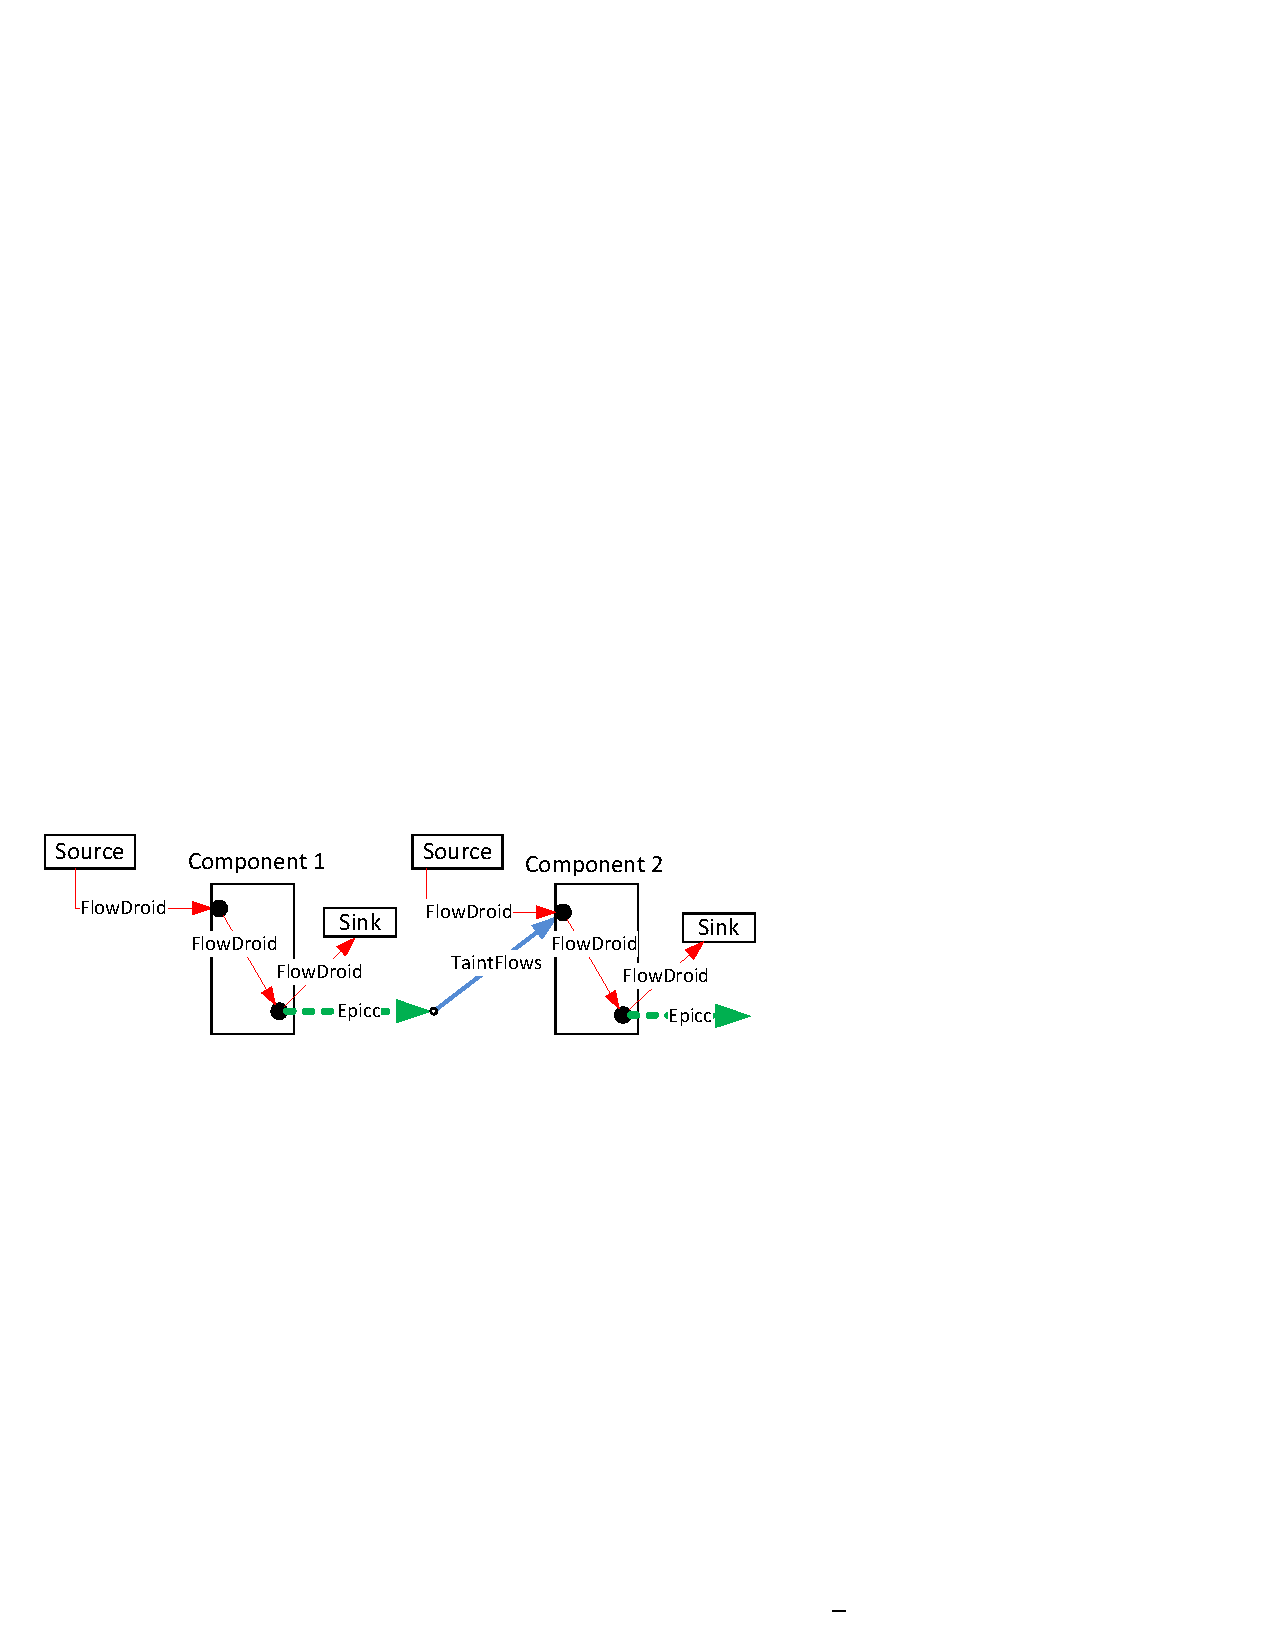
\includegraphics[trim = 5mm 100mm 85mm 140mm, clip, width=0.75\textwidth]{analysisPerDataFlowType_2comps.pdf}
\caption[Analysis by data flow type]{: FlowDroid identifies sources (including intents received), flow of the data within the component, and sinks (including intents sent). Epicc identifies characteristics of intents sent by a component. TaintFlows, the Phase-2 analyzer, matches sent intents to components which could receive the intent, using app manifest data and matching intent IDs from Epicc and FlowDroid. 
%A component could have zero or more sources, sinks, intents received, and intents sent.
From beginning to end, a given data flow can be internal to one component or traverse multiple components that can be in a single app or multiple apps.}
\label{fig:analysisPerDataflowType}
\end{figure}

The overview of our analysis method is shown in Figure~\ref{fig:analysisPerDataflowType}.
%
The goal of our analysis is to produce a set of all possible source-to-sink
flows within a set of Android apps.  
%%%NOTE: definitions in Intro (slightly different, too)
%% For our analysis, we
%% define {\em source}, {\em sink}, and {\em leak} as in prior work~\cite{fritz2013highly}: A source is a call to a method
%% that reads data from a shared resource and returns a non-constant
%% value. A sink is a call to a method which accepts at least one
%% non-constant data value and writes that data to a shared resource. A
%% leak is sensitivedata flow from a source to a sink.
%
Our taint flow analysis takes place in two phases.  In
Phase~1, each application is analyzed individually.  Received intents
are considered sources, and sent intents are considered sinks.
The output of our Phase-1 analysis, for each app, consists of 
(1) flows within each component, found by FlowDroid;
(2) identification of the properties of sent intents, as found by Epicc; and
(3) intent filters of each component, extracted from the manifest file.

An intent ID is assigned to every source code location that sends an
intent (i.e., a source code location that consists of a call to a method in the
\ttt{startActivity} family), as described in Section~\ref{para:apk-transformer}.
Sent intents with distinct IDs are considered distinct sinks, while intents with 
the same ID are combined together.


Phase~2 of the analysis is carried out on
a particular set of apps, using the output of Phase~1.
The output of Phase~2 consists of all the source-to-sink flows found in the
set of apps.
%
%In the rest of this section, we describe each phase in detail.
%
%% In Section~\ref{subsec:partsOfAnalyzer}, we detail how we implement our
%% analysis methods using FlowDroid and Epicc.
%% In order to test apps with
%% our method incorporating the most precise analysis tools, 
%% additional steps are needed, which are described in
%% Section~\ref{subsec:partsOfAnalyzer}. 

%\notes{I ignored figures for now. Please copy them back. }

\section{Example Scenario} \label{sec:example-scenario}
%\notes{Do these components belong to the same app or different app?
%(Answer: could be in same app or different apps, analysis the same)
%Can we say that epicc and flowdroid don't work for this example? If
%so, say it explicitly.}

\begin{figure}
\center
\scalebox{0.75}{\input{flow1b.pdf_t}}
\caption[Running example]{Running example described in Section~\ref{sec:example-scenario}. $R(I_i)$ denotes the response to intent $I_i$ (set using \ttt{setResult}).}
%\lujo{explain what the example shows}
\label{fig:flow1}
\end{figure}

We next introduce an example of information flows between several
components (Figure~\ref{fig:flow1}) that cannot be precisely analyzed
by existing tools.
%%The example shown in Figure~\ref{fig:flow1} is used throughout this
%%section.  
Suppose that Component $C_1$ sends data to Component $C_2$ and
receives data from it in return.  Component $C_3$ interacts with $C_2$ in a similar fashion.  We do not specify whether these three components belong to different apps or to a single app; the analysis is the same in either case.  As depicted in Figures~\ref{fig:flow1} and \ref{fig:intents-inflow-outflow}, for $i \in \{1,3\}$:
\begin{enumerate}
\item
    Component $C_i$ calls \ttt{startActivityForResult} to send data from source $\src_i$ to component $C_2$ via intent $I_i$.
\item
    Component $C_2$ reads data from intent $I_i$ and sends that data back to
    component $C_i$ by calling \ttt{setResult}.
\item
    Component $C_i$, in method \ttt{onActivityResult}, reads data from the result and writes it to sink $\sink_i$.
\end{enumerate}
%
To be precise, our analysis should determine that 
(1) information flows from $\src_1$ to $\sink_1$ (but not $\sink_3$),
and (2) information flows from $\src_3$ to $\sink_3$ (but not $\sink_1$).  
Note that FlowDroid by itself cannot produce this precise of a result, even in
the case where the three components are part of a single app.


\begin{figure}[b]
\center
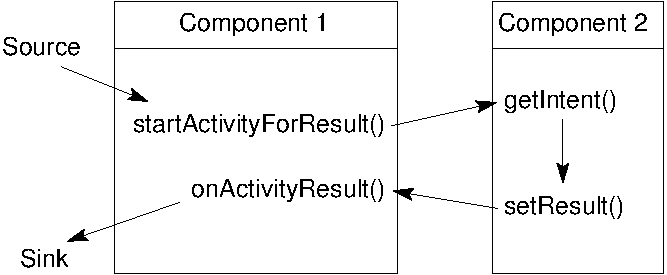
\includegraphics[width=0.6\textwidth]{small-in-out-flows.pdf}
\caption{Interaction between $C_1$ and $C_2$ in the running
  example}
\label{fig:intents-inflow-outflow}
\end{figure}
%\begin{figure}[!bt]

\def\ResultOf{R}
\def\IntentCons{I}
\def\Null{\tsf{null}}
\section{Phase 1} 
%\notes{There is no analysis
%  on flows within a component that is not by intent?}
In this phase, we analyze each app individually.  We identify an
intent by a tuple of (sending component, receiving component, intent ID).  
%As mentioned above, the intent ID is an identifier (unique within
%each app) assigned as described in
%section~\ref{para:apk-transformer} \lujo{does it matter how it's
%  assigned? if not, omit sentence; if yes, explain}.  
An intent sent from $C_1$ to
$C_2$ with ID $id$ will be denoted by $\IntentCons(C_1, C_2, id)$.

\begin{sloppypar}
In Phase 1, when a component calls a method in the \ttt{startActivity} family,
we do not know which components can potentially receive the the intent 
(because each app is analyzed in isolation in Phase~1, but potential recipients can
be components of other apps),
so we use $\Null$ for
the recipient field.  Likewise, in the \ttt{onCreate} method (which the Android
OS calls when the activity component receives an intent), we do not know
the sender of the intent, so we use $\Null$ for the sender field.
%% @Will: Carol commented here that null font different from other literals. Is that on purpose? Or, option below.
%\ttt{Null} for the sender field.
%
If a component receives an intent $I_1$ and returns information via
the \ttt{setResult} method, we denote the returned information by
$\ResultOf(I_1)$.  
\end{sloppypar}

We write $\mathit{source} \xrightarrow{C} \mathit{sink}$ 
%\lujo{please use \textbackslash{}mathit for words in math mode!} 
%WILL: @Lujo: This is automatically done by multiple-letter-spacing.tex.
to denote that information flows from
$\mathit{source}$ to $\mathit{sink}$ in component $C$.  For this purpose, we treat intents as
both sources (in the component that creates and sends the intent) and sinks (in
the component that receives the intent).  Using this notation, we represent
the flows depicted in Figure~\ref{fig:flow1} and described in
Section~\ref{sec:example-scenario} as follows:
%the desired results of the individual analyses of the apps in the running example
%as follows:
%
\begin{align*}
\src_1 & \xrightarrow{C_1} I(C_1, \Null, id_1)
\\
R(I(C_1, \Null, \Null)) & \xrightarrow{C_1} \sink_1
\\
I(\Null, C_2, \Null) & \xrightarrow{C_2} R(I(\Null, C_2, \Null))
\\
src_3 & \xrightarrow{C_3} I(C_3, \Null, id_3)
\\
R(I(C_3, \Null, \Null)) & \xrightarrow{C_3} \sink_3
\end{align*}
%
The above flows constitute the desired output of the FlowDroid analysis.
Although all the flows in the running example involve intents, in general our
analysis will also find flows from non-intent sources to non-intent sinks.

%\lujo{explain where these example results come from; at the moment,
%\wek{I changed the text to make it clearer.}

%We focus \lujo{in description or in implementation?} on intents sent and
We focus, in both description and in implementation, on intents sent and
received by \ttt{Activity} components; other types of components (services,
content providers, broadcast receivers) can be handled similarly.

\section{Phase 2} \label{sec:phase2}
After all apps in the given set have been analyzed, we enter Phase~2.
Our goal is to find out how tainted information can flow between components.
For each sent intent, we find all possible recipients, and
we instantiate the Phase-1 flow
equations (which have missing sender/receiver information) for all
possible sender/receiver pairs, as we describe in detail in
Section~\ref{subsec:gen-phase2-eqs}.
For the running example, the Phase-2 flow equations are as follows:
%\lujo{explain briefly why we generate these and why a reader should care}
\begin{align*}
\src_1 & \xrightarrow{C_1} I(C_1, C_2, id_1)
\\
R(I(C_1, C_2, id_1)) & \xrightarrow{C_1} \sink_1
\\
I(C_1, C_2, id_1) & \xrightarrow{C_2} R(I(C_1, C_2, id_1))
\\
I(C_3, C_2, id_3) & \xrightarrow{C_2} R(I(C_3, C_2, id_3))
\\
\src_3 & \xrightarrow{C_3} I(C_3, C_2, id_3)
\\
R(I(C_3, C_2, id_3)) & \xrightarrow{C_3} \sink_3
\end{align*}

\noindent
Let $T(s)$ denote the taint of $s$, that is, the set of sensitive sources from
which $s$ potentially has information. The goal of the analysis is to determine the taint of all sinks.
%% We first model taint flow over over single edges between pairs of components, using set equations to match components which can send and receive data. 
%% Then, we solve these equations in order to find all sinks which can be reached by each source, which 
%Each flow equation above relates the taint of the source of the flow to 
Each phase-2 flow equation $s_1 \to s_2$ relates the taint of $s_1$ to the taint of $s_2$. 
If data flows from $s_1$ to $s_2$, then $s_2$ must be at least as tainted as $s_1$.
Accordingly, we generate a taint equation $T(s_1) \subseteq T(s_2)$. For the running examples, the taint  equations we generate are:
%\lujo{explain briefly what's going on and why a reader should care.}
\begin{align*}
T(\src_1) & \subseteq T(I(C_1, C_2, id_1))
\\[0.4ex]
T(R(I(C_1, C_2, id_1))) & \subseteq T(\sink_1)
\\[0.4ex]
T(I(C_1, C_2, id_1)) & \subseteq T(R(I(C_1, C_2, id_1)))
\\[0.4ex]
T(I(C_3, C_2, id_1)) & \subseteq T(R(I(C_3, C_2, id_3)))
\\[0.4ex]
T(\src_3) & \subseteq T(I(C_3, C_2, id_3))
\\[0.4ex]
T(R(I(C_3, C_2, id_3))) & \subseteq T(\sink_3)
\end{align*}
Each non-intent source $s$ is tainted with itself, i.e.,
$T(s) = \{s\}$.
We then find the least fixed-point of the set of taint equations.
The end result of Phase 2 is the set of possible source to sink flows.
\def\ismatch{is\_match}

\subsection{Details of Generating Phase 2 Flow Equations} \label{subsec:gen-phase2-eqs}
Let $S$ be the set of sources and sinks (including intents and intent results)
in the Phase~1 flow equations. 
%
Consider a transmitted intent $I_{\rm TX}$ and a received intent $I_{\rm RX}$ from Phase~1.
In all cases, $I_{\rm TX}$ will have the form $I(C_{\rm TX}, \Null, id)$, and
$I_{\rm RX}$ will have the form $I(\Null, C_{\rm RX}, \Null)$.
%Let $\ismatch(I_{\rm TX}, I_{\rm RX})$ denote whether intent $I_{\rm TX}$
%matches the intent filter of component $C_{\rm RX}$, as described in Section~\ref{subsec:intent-resolution-rules}.

%Using the information from analyzing the apps separately, we construct equations which match data senders and receivers. 

In Section~\ref{sec:phase2}, we said that we instantiate the Phase-1 flow
equations for all possible intent sender/receiver pairs.  We now give the
details of how we do this.
For each Phase-1 flow $\src \to \sink$, we generate the set of all flows of the
form $\src' \to \sink'$ that satisfy the following conditions:
%\lujo{explain briefly what's going on and why a reader should care}
\begin{sloppypar}
\begin{enumerate}%[\setlength{\IEEElabelindent}{0pt}]
\item 
    If $\src$ is a regular (non-intent) source, then $\src' = \src$.
\item 
    If $\sink$ is a regular (non-intent) sink, then $\sink' = \sink$.
\item 
    If $\src$ has the form $I(\Null, C_{\rm RX}, \Null)$ (for example, the
    result of a call to \ttt{android.app.Activity.getIntent()}), then
    $\src'$ must have the form $I(C_{\rm TX}, C_{\rm RX}, id)$
    where there exists an intent $I(C_{\rm TX}, \Null, id) \in S$
    that matches the intent filter of component $C_{\rm RX}$.
%, as described in Section~\ref{subsec:intent-resolution-rules}.
\item
    If $\sink$ has the form $I(C_{\rm TX}, \Null, id)$ (for example, an intent
    object passed to \ttt{startActivity}), then
    $\sink'$ must have the form $I(C_{\rm TX}, C_{\rm RX}, id)$
    where component $C_{\rm RX}$ has an intent filter that matches the
    intent $\sink$.
%, as described in Section~\ref{subsec:intent-resolution-rules}.
\item
    If $\src$ has the form $R(I(C_{\rm TX}, \Null, \Null))$ (for example, a
    parameter of the callback method \ttt{onActivityResult}), then 
    $\src'$ must have the form $R(I(C_{\rm TX}, C_{\rm RX}, id))$ where 
    \begin{enumerate}
    \item
	there exists an intent $I(C_{\rm TX}, \Null, id) \in S$ that matches the
	intent filter of component $C_{\rm RX}$, and
    \item
	%there exists an intent result 
	$R(I(\Null, C_{\rm RX}, \Null)) \in S$.
    \end{enumerate}
\item
    If $\sink$ has the form $R(I(\Null, C_{\rm RX}, \Null))$ (for example, a
    value passed to \ttt{setResult}), then 
    $\sink'$ must have the form $R(I(C_{\rm TX}, C_{\rm RX}, id))$
    where
    \begin{enumerate}
    \item
	there exists an intent $I(C_{\rm TX}, \Null, id) \in S$
	that matches the intent filter of $C_{\rm RX}$, and
    \item
	$R(I(C_{\rm TX}, \Null, \Null)) \in S$.
    \end{enumerate}
\item
\label{it:receiverTaint}
    If $\src$ has the form $I(\Null, C_{\rm RX}, \Null)$ and
    $\sink$ has the form $R(I(\Null, C_{\rm RX}, \Null))$,
    then $\sink'$ must be $R(\src')$.
\end{enumerate}
\end{sloppypar}

Condition~\ref{it:receiverTaint} allows us to precisely handle a situation in
which a component (such as $C_2$ in the running example) processes data from
various callers without intermingling the taintedness of the data.  
Condition~\ref{it:receiverTaint} is sound as long as multiple instances of the
component can communicate only via flows included in the Phase-1 equations.
Our current implementation catches most such flows but misses inter-instance
communication via static fields.  

For example, in Figure~\ref{fig:flow1},
if all components are part of the same app, then the two launched instances of
$C_2$ can store information from $I_1$ and $I_3$ in a static field (which is
shared between the two instances of $C_2$).  The value in the static field
(tainted with both $src_1$ and $src_3$) can then be read and copied into
$R(I_1)$ and $R(I_3)$.  This flow would be missed by our current analysis.


For future work, we plan to address static fields in a sound manner.  In
particular, if an app $A$ has a class $C$ with a static field $sf$, we would
modify FlowDroid to introduce a dummy entity $sf\!_{A , C}$ that can act both as a
source and as a sink.  Reading from static field $sf$ would be treated as
reading from $sf\!_{A,C}$, and writing to $sf$ would be treated as writing to
$sf\!_{A,C}$.  The resulting Phase-1 flow equations would enable our Phase-2
analysis to soundly handle inter-instances communication via static fields.

\begin{figure}[!bt]
\center
\scalebox{0.80}{\input{flow2.pdf_t}}
\caption[Example of inter-app communication flow]{ wherein, for $i \in \{1,3\}$: $C_{\rm 2a}$ receives tainted data from $C_i$, sends it to $C_{\rm 2b}$, receives a result with the same taint, and finally sends it back to $C_i$.
}
\label{fig:flow2}
\end{figure}
Our analysis cannot precisely handle the situation in
Figure~\ref{fig:flow2}, wherein tainted data travels through a chain of apps.
In this situation, our analysis would mark all intent results as being tainted
with data from both $I_1$ and $I_3$ instead of being able to keep them separate.
%There are various ways of changing the analysis to precisely handle the
%situation in Figure~\ref{fig:flow2}, involving varying trade-offs between speed
%and precision.  


\subsection{Rules for Matching Intents} \label{subsec:intent-resolution-rules}
%\lujo{this subsection appears with no warning and no context is given
%  for how it fits in with the rest. fix this. add to previous subsection?}
In Section~\ref{subsec:gen-phase2-eqs}, we used the term
``match'' in relation to a sent intent and an intent filter.  We now more
fully define what we mean by ``match''.
The Android
documention\footnote{\url{http://developer.android.com/guide/components/intents-filters.html\#Resolution}}
describes how a sent intent is matched to potential recipients.
If the intent explicitly designates a recipient, then the intent is
matched with exactly that recipient.  Otherwise, the intent is matched with a
filter if it passes three tests: an action test, a category test, and a data
test. 

Epicc provides information about outgoing intents in its app analysis, and we use that. 
It provides no information about the URI
fields of intents, so we ignore the URI fields when matching intents with
intent filters. 
%\lujo{why are we talking about Epicc all of a sudden,
%  when so far the analysis has been described completely in the
%  abstract (i.e., with no mention of FlowDroid or Epicc)? either don't
%mention these tools anywhere, or mention them {\bf briefly} throughout Sec 3}

Sometimes, Epicc will return \ttt{<any\_string>} for the action string or
{\ttt{Found top element} for the intent as a whole.  For this case, the analyzer
has two modes (which can be selected by a command-line option): 
(1) a sound mode, which assumes that an unknown action string potentially
matches any action string in any filter, thereby typically generating many
false positives, and 
(2) a precise mode, which assumes that the unknown action string doesn't match
any filter, thereby potentially generating false negatives.  
Likewise, in the sound mode, a top-element intent matches every filter, and in
the precise mode, it matches nothing.

%%%%%%%%%%%%%%%%%%%%%%%%%%%%%%%%%%%%%%%%%%%%%%%%%%%%%%%%%%%%%%%%%%

%%%%%%%%%%%%%%%%%%%%%%%%%%%%%%%%%%%%%%%%%%%%%%%%%%%%%%%%%%%%%%%%%%

\chapter{Implementation Details} \label{sec:test}
We have implemented our approach
%\notes{review rest of paragraph: a few high level sentences} 
in an analyzer 
%that runs Epicc and a modified FlowDroid and uses the
%output of those analyses to perform a taint analysis, which includes
%intercomponent communication via intents \lujo{redundant--these tools
%  do this anyway; what's new?}.
%We call our implementation 
that we call ``DidFail'' (Droid Intent Data Flow Analysis
for Information Leakage).
% We used DidFail to test a set of apps.
%
Our analyzer (source code and binaries), along with 3 apps which demonstrate
the running example in \S\ref{sec:example-scenario},
%, which match the examples in Section \ref{sec:analysis}, 
is available at: \url{http://www.cert.org/secure-coding/tools/didfail.cfm}
%\begin{center}\url{http://www.cert.org/secure-coding/tools/didfail.cfm}\end{center}
%\limin{Why some of the apps? Have to be precise here.}
%The three apps which demonstrate the running example in this paper are included, with others.
%Due to copyright restrictions, we can only provide download information about some of the apps.

%\notes{Review: Organize this section closer to phase 1 and phase 2. A high-level diagram would be useful}
%\section{Implementation of the Analyzer} \label{subsec:partsOfAnalyzer}
%%%% Here, enter text to describe parts of our analyzer used for testing
\begin{figure}[b!]
\center
%\par
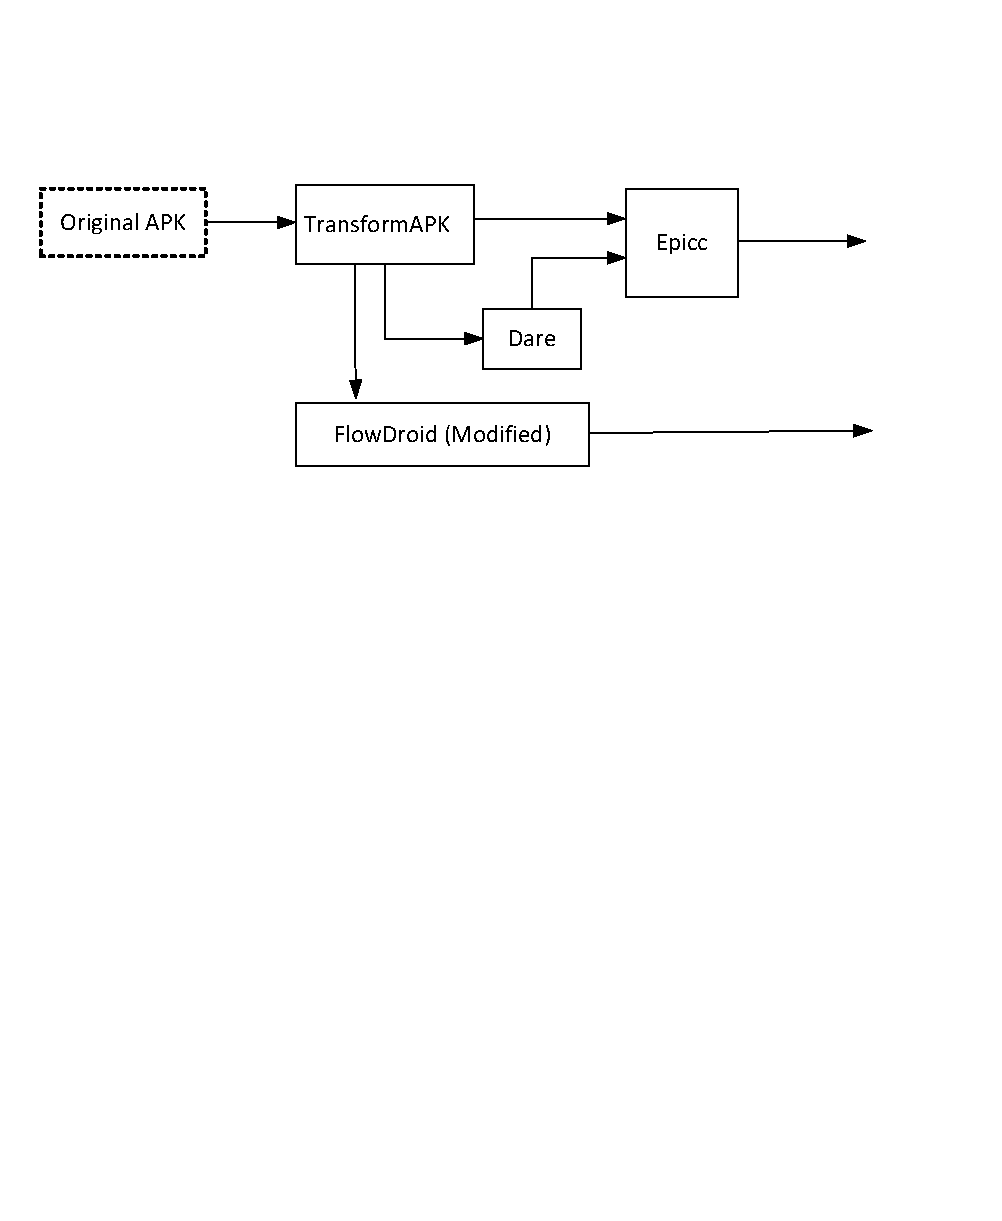
\includegraphics[trim = 5mm 125mm 10mm 25mm, clip, width=0.75\textwidth]{phaseOne_v9.pdf}
\caption{Phase 1}
\label{fig:phase1}
%%\begin{figure}[!h]
%%\center
%%\par
%\includegraphics[trim = 5mm 145mm 25mm 20mm, clip, width=0.50\textwidth]{dataFlowBothPhases_1_N.pdf}
%\caption{Data Flow Including Phase 1 and Phase 2
%%\limin{this figure can be shrink in half if we need space. just keep app1 and appn, and remove unnecessary white space.}
%}
%\label{fig:phase2etc}
%%\end{figure}
\end{figure}

\section{Phase 1 Analysis}\label{subsec:phase1}
Figure \ref{fig:phase1} %and  \ref{fig:phase2etc} 
show the components of
our analyzer, the processing sequences, and dataflow
paths. The analyzer incorporates use of the previously
existing and unchanged tools Epicc, Dare, and Soot; a modified
version of FlowDroid; and new tools TransformAPK and TaintFlows.
%The run-didfail program runs the full analysis, calling
%tools in the order shown in the figures. 
TaintFlows performs the Phase 2 analysis.%, as described in Section \ref{sec:analysis}.
%, and also parses each app's manifest file (part of Phase 1). 
%Didn't name each new script here. Should we add more?
%\lujo{say what TransformAPK does}
\subsection{APK Transformer} \label{para:apk-transformer}
The APK Transformer must be used in the first step of the analysis, in order to be able to integrate results of the different analytical tools used afterwards. This step was critical in order to achieve our ultimate goal of outputting detected paths from sources to sinks, including paths which contain dataflows via intents.
Android apps are packaged in files with the extension {\em.apk}. 
In Figure \ref{fig:phase1}, ``Original APK'' is the original Android app. With the APK Transformer, our analyzer modifies that app to enable matching intents mentioned in both the Epicc and FlowDroid outputs. 
To do this, we transformed each original .apk file into a modified
.apk file, using Soot. 
%%~\cite{bodden2013easily}. 
We wrote a program that first uses Soot to transform the .dex Android
bytecode into an intermediate representation called {\em jimple}. The
program uses the Soot framework to locate method calls that send
intents, and immediately before that, we insert new jimple code, which
calls an Android method that inserts a unique ID into the
intent. Then, our program uses Soot to compile the modified jimple
code into a new .apk file. When Epicc processes this modified file, it
prints the unique intent IDs.  
%\limin{shouldn't reference 4.1.1 in  4.1.1. please fix.}  
%% \limin{The following text needs to be  re-organized. Are you trying to explain why APK transformer is
%%   needed for FlowDroid and Epicc? why do you need to mention how to
%%   modify the source of FlowDroid? what's the relation here?  Maybe
%%   it's better to write the paragraph for Epicc first?}  
As described
in Section \ref{para:fd_mod}, we modified the source code of FlowDroid
so that its output identifies sent intents by their intent ID,
%to output the new field name for each intent, 
enabling us to match
intent analysis from the two tools. We could not modify the source code of Epicc, because it is currently
published only as a .jar file. 
%This .apk transformation is done because we could not
%modify Epicc code to match particular intents from the output of the
%two tools. 
According to the Epicc website, the authors plan to publish
the source code in the future. 
After the source code is available, we might be able to combine FlowDroid and
Epicc in a more efficient manner.

%After that, we could modify the Epicc
%tool to print unique intent IDs, which would speed our analysis
%because the extra .apk transformation would be unnecessary.



\subsection{FlowDroid (Modified)} \label{para:fd_mod}
We modified FlowDroid in several ways. For our Phase-1 analysis, we consider the points where intent information flows in and out of the component as sources and sinks respectively. 
Therefore, we added the method \ttt{onActivityResult()} as a source and
\ttt{setResult()} as a sink in FlowDroid. The methods \ttt{getIntent()} and \ttt{startActivityForResult()} were already present as a source and sink respectively.
%Therefore, we added the methods \ttt{getIntent()} and \ttt{onActivityResult()} as sources and \ttt{startActivityForResult()} and \ttt{setResult()} as sinks in FlowDroid. 
Although the FlowDroid tool comes with a smaller  \ttt{SourcesAndSinks.txt} file, one can substitute the much larger \ttt{SourcesAndSinks.txt} file from the SuSi analyzer~\cite{rab14classifying}\footnote{{https://github.com/secure-software-engineering/SuSi} (2013-11-25)}.
%% \TODO{
%% \begin{itemize}
%% \item delete 2 methods since now covered by SourcesAndSinks.txt, if FlowDroid works ok with that
%% \item Remove sentence with footnote above, if final test does not use longer SuSi file
%% \end{itemize}
%% }
We also added code to look for the \ttt{putExtra} call we added to insert the unique intent ID, which was added by the APK Transformer.
In flows where an intent is the sink, the output of FlowDroid identifies the intent by its unique ID.
%When that call is found, the intent's unique ID is stored in a data structure that is accessed when printing out dataflows between sources and sinks that FlowDroid found. The unique ID gets printed if the FlowDroid sink (for this component) is a sent intent. % This last line of the paragraph needs modification

\begin{sloppypar}
In a flow $src \xrightarrow{C} I(C,\Null,id)$, how do we identify $C$?
%Our implementation currently does not this in all cases.\footnote{%
When an intent is sent via \ttt{base.startActivity} (including the case where \ttt{base} is an implicit \ttt{this}), we assume that
that the class of \ttt{base} must be
the sending component.\footnote{%
We have not yet been able to confirm or refute whether this is 
a sound assumption.  
%As a quick and dirty solution, we decided to do without identification of the component.
To preserve soundness at the expense of precision, we considered an intent as
potentially matching the intent filter of all components of an app if it matches
the intent filter of any component of the app.
}
\end{sloppypar}
%There are three cases.  First, if $src$ has the form $I(C_3, C_1, id_B)$, then
%$C_1$ is the class with the member function \ttt{getIntent} from which the
%tainted data is obtained. 
%Second, if $src$ has the form $R(I(C_1, C_3, id_B))$, then $C_1$ is the class
%with the callback member function \ttt{onActivityResult} to which the 
%tainted data is passed as a parameter.
%Third, if $src$ has any other form, then the precise identity of $C_1$ doesn't really matter for the purposes of the Phase~2 analysis (unlike the first two cases, where ), and we do not attempt to identify $C_1$; instead, we just put the app package name in the $C_1$ field.


The output of FlowDroid 
%\cite{soot-vallee-master-thesis}
was originally
non-deterministic in the order in which flows were listed.  To produce
deterministic output for regression testing, we simply sorted the flows before
printing.% the output.


\subsection{Epicc and Dare} \label{para:epiccAndDare}
The Dare \cite{octeau2012retargeting} tool takes the transformed .apk file as
input, retargets the application, and outputs Java class files.
The Epicc analysis takes two inputs: the transformed .apk file and the output of Dare.


\section{Phase 2 Analysis} \label{subsec:phase2}
%Figure \ref{fig:phase2etc} shows the relationship of the analyses in Phase 1 and Phase 2.
Each app in the app set undergoes its own separate Phase-1 analysis, with each Phase-1 analysis output providing three separate output files (manifest file, Epicc output and FlowDroid output) that are input to the Phase-2 analysis. If there are $n$ apps in the app set, then the Phase-1 analysis is performed $n$ times, outputting $3n$ files, all of which are input to the (single) Phase-2 analysis. The Phase-2 analysis output provides information about dataflows from a source to a sink, including intents if they are part of the data flow.
%More detail needed on phase 2 output.


\chapter{Experimental Results} \label{subsec:experimental}
We tested our prototype analyzer on two app sets. App Set 1 contains 3 apps that we created, which match the running example in Figure~\ref{fig:flow1}.  App Set 2 contains 3 apps from the DroidBench benchmark suite \cite{ecspride2014droidbench} that use intents for inter-app communication.
Our analyzer successfully traced all inter-app and intra-app flows in both app sets. As described in the previous section, we first ran the Phase 1 analysis on all apps individually, and then we ran the Phase 2 analysis for each set of apps.

\begin{figure}
\center
\vspace{-2ex}
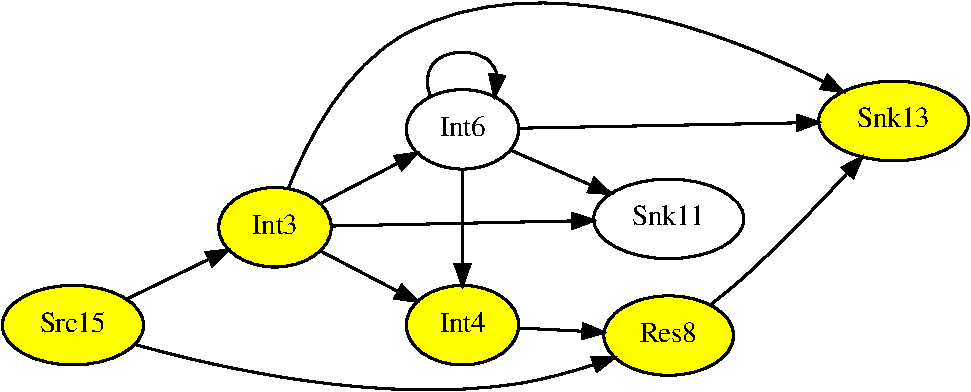
\includegraphics[width=0.6\textwidth]{droidbench-graph-crop.pdf}
\caption[Tainted data flow in DroidBench apps]{.  
Graph created by running Graphviz on output of our analyzer.
Src15=\ttt{getDeviceId}, 
Int3=I(IntentSink2,IntentSource1,3),
Int4=I(IntentSource1,IntentSink1,4), 
Res8=R(Int4),
Snk13=\ttt{Log.i}
}
\label{fig:droidbench-graph}
\end{figure}

\paragraph{App Set 1}
\begin{sloppypar}
\begin{itemize}
\item
SendSMS.apk: This app leaks the user's DeviceId through an SMS. It reads the user's DeviceId, then adds it to an intent using the \ttt{putExtra} method. It then sends this intent out by calling \ttt{startActivityForResult}. Another app receives this intent and responds with a result. When the intent result is received, the \ttt{onActivityResult} callback method is called. Data received in the result is then leaked through an SMS.
\item
Echoer.apk: This app receives intents from other apps. It reads the incoming intents using the \ttt{getIntent} method, and writes the received data using \ttt{Log}. Also, it sends this data back to the transmitter using the \ttt{setResult} call.
\item
WriteFile.apk: This app is similar to SendSMS except that it reads the user's location and leaks it to the FileSystem.
\paragraph{Result:}
Our analysis detected the following interesting flows:
\begin{flushleft}
\begin{itemize}[leftmargin=*]
\item
$getDeviceId \xrightarrow{SendSMS} startActivityForResult $
%\xrightarrow{AppC2} 
\\
$getIntent \xrightarrow{Echoer} setResult $
\\
$onActivityResult \xrightarrow{SendSMS}sendTextMessage$

\item 
$getLastKnownLocation  \xrightarrow{\!WriteFile\!} startActivityForResult  $
%\xrightarrow{AppC2} 
\\
$getIntent  \xrightarrow{Echoer} setResult  $
\\
$onActivityResult  \xrightarrow{WriteFile} write$
\end{itemize}
\end{flushleft}
\end{itemize}
\end{sloppypar}

\paragraph{App Set 2: Droidbench Benchmark Suite}
\begin{sloppypar}
DroidBench is a set of open source apps for testing static analysis tools.
\begin{itemize}
\item
IntentSource1.apk: This app reads the incoming intent using \ttt{getIntent}, and sends the intent out by calling \ttt{startActivityForResult}. When another app receives this intent and responds with a result, this app logs the result (Sink).
\item
InterAppCommunication\_IntentSink1.apk: This app read the user's DeviceId (Source), adds it to the received intent, and then sends the intent out by calling \ttt{getIntent} method.
\item
InterAppCommunication\_IntentSink2.apk: This app also reads the user's DeviceId (Source), adds it to a new Intent object, and sends the intent out by calling \ttt{startActivty}.
\paragraph{Result:}
Our analysis detected the following interesting data flows as shown in the Figure \ref{fig:droidbench-graph}.
\begin{flushleft}
\begin{itemize}
\item
$Src15  \xrightarrow{IntentSource1} Int3 \xrightarrow{IntentSource1} Snk13$
\item
$Src15 \xrightarrow{IntentSource1} Res8 \xrightarrow{IntentSource1} Snk13 $
\end{itemize}
\end{flushleft}
\end{itemize}
Note: The apps InterAppCommunication\_IntentSink1 and InterAppCommunication\_IntentSink2 use the same package name `de.ecspride'. Since Android does not allow two packages with the same name, we changed the package names to `de.ecspride.IntentSink1' and `de.ecspride.IntentSink2'.
\end{sloppypar}


% Lori: @Will @Amar Need experimental results
%\TODO{Enter test results:
%\begin{itemize}
%\item InsecureBank
%\item MadRabbit
%\item Hugo Runner (if interesting results)
%\item Samsung's Push Service (if interesting results)
%\end{itemize}
%}



%%%%%%%%%%%%%%%%%%%%%%%%%%%%%%%%%%%%%%%%%%%%%%%%%%%%%%%%%%%

%%%%%%%%%%%%%%%%%%%%%%%%%%%%%%%%%%%%%%%%%%%%%%%%%%%%%%%%%%%


\chapter{Sources of Unsoundness and Imprecision}\label{sec:soundness}\label{subsec:sources}
Among its sources of unsoundness and imprecision, our analysis inherits those from its building blocks, Epicc and FlowDroid.
%\limin{add the name of one more tool?}
% and the other parts of the DidFail analyzer. 
% Certain sources of unsoundness and imprecision have been discussed in
% Section \ref{subsec:intent-resolution-rules}. 
%\noindent\paragraph{Unsoundness}\label{subsec:unsoundness}
\paragraph{Unsoundness}\label{subsec:unsoundness}
Sources of unsoundness cause the analysis to fail to identify a tainted
flow.
%and how we connect them... including current version not having the more precise intent-to-in-component dataflow tracking planned for future
Sources of unsoundness in our analysis include reflection and native
code, which are not addressed by Epicc. FlowDroid also does not
consider reflective calls. %, so this is a source of unsoundness.
However, FlowDroid does analyze calls that invoke native code, using a heuristic
called {\em Taint Wrapping}.
It defines explicit taint propagation rules for commonly called native
methods. For all other native methods, FlowDroid uses the following heuristic:
if the input array was tainted before the call, then FlowDroid determines that all call arguments and any return
 value are tainted. 
 %\limin{check the previous sentence.}
% FlowDroid determines all call arguments and return
% values to be tainted. 
%
FlowDroid's handling of native calls is not
sound; it does not analyze the native code in the callee. 
For example, native code can read from sources and write to sinks, which
will not be detected by FlowDroid.
%\limin{why not analyzing the native code in the callee is a problem, if I already declare the return value being tainted anyway? clarify?}
%
FlowDroid also is unsound because it does not trace some leaks caused by multithreading and some implicit flows.
%FlowDroid's taint flow analysis ignores some implicit
% flows where the tainted data is not directly transmitted, and in those
% cases the resulting analysis is not sound.
% Limin: I comment this out because we have not talked about implicit
% flows at all
%probabilistic and possibilistic leaks caused by multi-threading
%Another source of unsoundness is from incomplete modeling of
%components' life cycles by Epicc or FlowDroid. 
%\limin{Give an example here. to support the arguement}
If the component's life cycle is not modeled completely by Epicc and/or FlowDroid, that would be another source of unsoundness, as discussed in FlowDroid~\cite{FlowDroid-PLDI-2014} and Epicc~\cite{octeau2013effective} papers.%For instance, if the Android lifecycle contained callbacks they are not aware of.

%% Discussion of implicit flows {
The analysis that we have presented does not consider implicit flows that
involve the mere receipt of intents without reading any information from the
received intents.  For example, suppose an app $A_T$ wants to communicate a bit vector 
$\tup{b_n, ..., b_0}$ to an app $A_R$ without being
detected by our analysis.  App $A_R$ can have two components, $C_{R0}$ and $C_{R1}$, 
which have mutually exclusive intent filters.
Then $A_T$ can send a sequence of intents $\tup{I_n, ..., I_0}$ where 
\begin{itemize}[topsep=0.25ex,itemsep=0ex,parsep=0ex]
\item intent $I_i$ matches $C_{R0}$ iff $b_i = 0$, and
\item intent $I_i$ matches $C_{R1}$ iff $b_i = 1$.
\end{itemize}
To ensure that intents arrive in proper order, App $A_T$ can use
\ttt{startActivityForResult} to send the intent and then wait until $C_{R0}$ or
$C_{R1}$ calls \ttt{setResult} to acknowledges receipt.
%% }

%Data can flow between components of different apps via file or database accesses such as writes to and reads from shared external storage (e.g., a connected computer, a removable SD card, and an internal non-removable storage device), internal storage which is MODE\_WORLD\_READABLE or MODE\_WORLD\_WRITEABLE, and `shared public directories on the device such as 'Music/','Pictures/', and 'Ringtones/'. These same file and databases can be accessed to allow (and sometimes to restrict) data flow between components of a single app. For instance, the internal file storage mode MODE\_PRIVATE restricts file access to a single app.
Data can flow between components of different apps via file or database accesses such as writes to and reads from shared external storage, 
% External storage sometimes is stored internal to the device
%(e.g., a connected computer, a removable SD card, and an internal non-removable storage device), 
internal storage, and shared public directories on the device. These same file and databases can be accessed to allow (and sometimes to restrict) data flow between components of a single app. 
FlowDroid considers a read from a file to be a source and a write to a file to be a sink. Within one component, the FlowDroid analysis finds a tainted flow if there is a read from a file and a call to a sink, or a call to a source and a write to a file. 
%However, a single write to a file from one component or app and a single read from another is a cross-component (possibly also a cross-app) taint flow that FlowDroid does not recognize. 
Although our analyzer finds some tainted flows, including file access, which FlowDroid does not, it does not soundly analyze taint flows involving files accesses.
Our analysis finds a multi-component tainted dataflow that ends with a write to a file sink. However, it does not trace a multicomponent tainted dataflow that starts with a read from a file source. Also, our analyzer is unsound because it does not trace a multi-component tainted dataflow with a read from a file in one component after a write to it by another.
%I think reads from a file are considered sources and writes to a file are considered sinks. Need to make sure same in tool as in their paper, so we should check SourcesAndSinks.txt
%Add: Discussion of Content Providers as components accessed with URIs which can be passed in intents. URIs aren't currently handled by Epicc, so taint flow across componenets via intents with URIs is not sound 

Additional sources of unsoundness in the analyzer include shared static fields. 
FlowDroid traces tainted data within a component (or within an entire app, depending on command line arguments) that is written to and/or read from a shared static field. 
Unsoundness due to inter-instance static field communication is discussed in Section~\ref{subsec:gen-phase2-eqs}. 
%% Within an app, different components can write to shared static fields and read from them, thus enabling a tainted dataflow to pass, which might eventually be sent to a sink. 
%% However, we use FlowDroid analysis only within a single component, and not to trace the flow of inter-component shared static field tainted data within an app.
%% However, FlowDroid analyzes only a single component, and does not trace the flow of inter-component shared static field tainted data within an app. 
%Reads from a static field *not* considered sources by FlowDroid, right? Check SourcesAndSinks.txt
%% Epicc intent analysis does not include consideration of shared static fields. 
%% TODO: Investigate above 2 lines
%% \limin{has the following been explained before? if not move the figure
%% to here}
%% Consider that all the components in Figure \ref{fig:flow2} are in the same app. Say $C_1$ calls a source $\src_1$ and then writes to a shared static field, then $C_3$ reads from that shared static field and then sends to a sink $\sink_3$. No phase 1 equation is generated for the source to (shared static field) recipient dataflow, nor for the flow of data from the shared static field to component $C_3$. Phase 1 equations can include only a source, a sink, an intent, or an intent result. Without phase 1 equations, no phase 2 equation gets created. This example demonstrates that our taint flow analysis is not sound with respect to shared static fields.
%% Another example which our prototype analyzer does not soundly analyze involves sensitive data flowing through a path that includes both shared static fields and an intent.
%% Say that in Figure \ref{fig:phase1}, components $C_1$, $C_2$, and $C_3$ are in different apps and $C_3$ has a shared static field $SF_X$. $C_1$ calls a source $\src_1$, and then sends that data to $C_2$ in an intent. $C_2$ writes that value to $SF_x$. After that, $C_2$ calls the \ttt{setResult} method and the $\src_1$ -tainted data is sent back to $C_1$. Similarly, $C_3$ calls a source $\src_3$, and then sends that data to $C_2$ in an intent. $C_2$ writes that value to $SF_x$. After that, $C_2$ calls the \ttt{setResult} method and the $\src_3$ -tainted data is sent back to $C_3$.

% FlowDroid captures sharedPreferences only as a sink, not as a source. Refer to SourcesAndSinks.txt file
\noindent\paragraph{Imprecision} \label{subsec:imprecision}
Imprecision in the analysis would result in the analysis
reporting a possible tainted flow where such flow is not
actually possible. For instance, the Epicc analyzer over-approximates
inter-component communication (ICC) because it does not handle URIs,
which are used by Android to match intents to receiving components. 
%Only the Epicc output regarding MIME data type is used to match sent intents to data elements of components' receiving filters, so our analyzer over-approximates possible receivers of intents carrying tainted data. If the sent intent has a URI, its URI must match a component's receive filter in order to be received, including and beyond the receive filter matches for the MIME type.\footnote{\url{http://developer.android.com/guide/components/intents-filters.html\#DataTest}}
As described above, FlowDroid's analysis of native calls is not precise and sometimes over-approximates returned tainted fields. 
Our analyzer does not use permissions to restrict possible matching of intent senders and receivers. This over-approximated matching is a source of analysis imprecision.

In our Phase-1 FlowDroid analysis, all the received intents for a component are
conflated together as a single source.  As future work, to be more precise, 
we plan to modify FlowDroid so that, when a callback function such as
\ttt{onCreate} is analyzed, it can report the data flows as a function of the
properties of the received intent. For example, we might report that
a component $C$ has a flow $camera \xrightarrow{C} R(I)$ iff 
$I.hasExtra(\qt{\ttt{cam}}) = \tsf{true}$.
Similarly, we can make analysis of \ttt{onActivityResult} be sensitive
to the value of the \ttt{requestCode} parameter.
%$$\ttt{if (i.action $=$ "cam") \ttc{x\;:=\;readCam();} else \ttc{$\ldots$}}$$

%\noindent
%\TODO{
%\begin{itemize}
%\item Discuss \ttt{requestCode} in \ttt{startActivityForResult} and \ttt{onActivityResult}.
%\item Future work: more precise handling of distinct incoming intents, treating them as distinct sources
%\item Discuss SOOT experience: non-deterministic, make final output deterministic by sorting
%\end{itemize}
%}


%%%%%%%%%%%%%%%%%%%%%%%%%%%%%%%%%%%%%%%%%%%%%%%%%%%%%%%%%%%%%%%%%%

%%%%%%%%%%%%%%%%%%%%%%%%%%%%%%%%%%%%%%%%%%%%%%%%%%%%%%%%%%%%%%%%%%


\vspace{-1.0ex}
\chapter{Related Work}
\label{sec:related-work}

The Epicc tool performs the most precise static analysis of Android intents of
any Android analyzer known to us, finding vulnerabilities with far fewer false
positives than the next best tools. 
%The analysis is fast, averaging only 113 seconds. %\TODO{This isn't meaningful without saying what the set of tested apps were and what the machine used was.}
The authors showed that the intent ICC
problem can be reduced to an inter-procedural Distributive Environment (IDE)
problem, so the  existing algorithms for efficient IDE solutions could be used.
Epicc builds on a pre-existing IDE framework within the Soot library.

Daniel Hausknecht's 2013 thesis \cite{hausknecht2013master} describes VarDroid,
intended to integrate intra-component and inter-component static analyses,
similar in some ways to our method. 
His concept is modular where different analyses could be switched out for the
intra-component and inter-component dataflow tracing. 
Where we use a modified FlowDroid, his concept could use Chex
\cite{lu2012chex}, FlowDroid, or another analyzer. His thesis says he did not
complete integrating FlowDroid in his system.  Instead, he simulated dataflow
analysis through probabilistically generated information simulating results of
the intra-component and inter-component analyses.
%\TODO{From my limited knowledge, it seems that his thesis doesn't actually analyze any Android (source|byte)code, he just generates fake data and does some analysis on that.  If this is true, we should emphasize it more.}
%Did he publish after this? 
%Could also add discussion of call graph creation, DFS or BFS, and efficiencies he discusses.

The Kirin tool \cite{enck2009understanding} provides a formalized model for stating data policy and compares stated policies to information extracted from app manifest files, processing this information on the phone, to determine whether an app should be installed.
%Our analysis (once further developed) versus theirs: much more precise policy analysis possible. An indicator!: their analysis is able to use the limited memory and processing of the phone, and ours needs much more.\noindent\paragraph{Unsoundness}\label{subse:unsoundness}
The SORBET \cite{fragkaki2012modeling} system modified a standard Android system to enable formal definition of desired security properties, which were proven to hold on SORBET but not on Android. 
%SORBET additions were made to the kernel, the Java API, and new data structures were added beyond what exists in Android: Sorbet Static Data storage, a Sorbet Reference monitor within the Android Activity Manager, and Instance Data. 
Livshitz et\ al.~\cite{livshits2005finding} did static analyses on Java code to detect policy violations with security implications, including taint analysis.
TaintDroid~\cite{enck2010taintdroid} does realtime taint tracking to dynamically detect data leaks. 
%%%%% TODO: Need discussion of ScanDroid 

Felt et\ al.~\cite{felt2011android} found that about one-third of Android apps (of the 940 they tested) asked for more privileges than actually used. They found evidence that a cause of over-privilege is developer confusion in part due to insufficient Android API documentation. Furthermore, malicious apps can use permission re-delegation attack methods \cite{felt2011permission}, which when successful take advantage of a higher-privilege app performing a privileged task for an application without permissions. The ComDroid \cite{chin2011analyzing} tool analyzes inter-app communication in Android, looking at intents sent and the manifest files for potential vulnerabilities due to app communication. Although it examines vulnerabilities due to intents, the ComDroid analysis does not trace and identify data paths between sources and sinks.
%% McAfee's mobile security report released in February of 2014~\cite{mcafee2014whos} provides results from their study of sensitive data collected by apps, reporting they found $80\%$ of Android apps collect location information ($55\%$ continuously track location), $82\%$ read the device ID, and $26\%$ know the device sim card number. 
%%  Sensitive data should be protected against leaking to unprotected or undesired locations. For desired functionality, users need some types of sensitive data to flow between apps. However, analysis of data flows is necessary in order to determine that sensitive data remains within secure and expected boundaries. Some apps are malicious and try to steal data or to alter sensitive data, sometimes using multiple colluding apps. Other apps allow sensitive data to flow to an unprotected location through coding errors. 
%% For desired functionality, users need some types of sensitive data to flow between some apps. 
%%%%%%%%%%%%%%%%%%%%%%%%%%%%%%%%%%%%%%%%%%%%%%%%%%%%%%%%%%%%%%%%%%
%%%%%%%%%%%%%%%%%%%%%%%%%%%%%%%%%%%%%%%%%%%%%%%%%%%%%%%%%%%%%%%%%%
\chapter{Conclusions and Future Work} \label{sec:conclusions} This
paper introduced a new analysis that integrates and enhances
existing Android app static analyses in a two-phase method.
We demonstrated feasibility by 
implementing our approach 
%creating a prototype analyzer 
and testing apps with it. Future work planned includes enhancing the inter-component
part of the taint flow analysis to include additional data channels
such as static fields, SQLite databases, and SharedPreferences. 
%When the Epicc tool's source code is published, we plan to simplify and
%speed up our prototype analyzer, by eliminating the TransformAPK tool
%and inserting the unique intent IDs within a modified Epicc.  
We also plan to test a large number of publicly available Android apps.
We envision that a two-phase analysis such as ours can be used as follows.
An app store can run the Phase-1 analysis on each of the apps in the app store.
When a user wants to install a new app, the app store would conduct the Phase-2
analysis and tell the user about the new flows that would be made possible if
the new app is installed.

%\TODO{Write sentence about app store. E.g., app store can run Phase-1 analysis on apps, then when use wants to install a new app, the app store (or user's phone) conducts Phase-2 analysis and tells user about all the possible flows.}

% Lori: @Will @Amar Conclusions needed

%% \appendix
%% \section{Appendix Title}
%% This is the text of the appendix, if you need one.

%\acks

